\chapter{Implementation Details}
In this chapter it is provided a more in depth explanation of how the different functionalities have been implemented in this project. The main operations that have been added to the L1 API for managing the PUFs are:
\begin{itemize}
	\item Fill the DB with a number of responses
 	\item Perform a challenge and determine the authenticity of the device  
\end{itemize}

To perform these actions correctly a communication between the Host and the Board is necessary. 

The board is responsible for:
\begin{enumerate}
	\item Reading the PUF responses from the RAM and store them in the flash;
	\item Providing the list of all PUF responses to the host;
	\item Returning a specific response corresponding to the challenge sent by the host.
\end{enumerate}

On the other hand, the host is in charge of:
\begin{enumerate}
	\item Retrieving the list of PUF responses and storing them in a database;
	\item Sending a challenge to the board, retrieve the response to that challenge and then compare it with the one stored in the database.
\end{enumerate}


\section {PUF retrieval and DB initialization}
At the beginning it is necessary to access the RAM as soon as possible to avoid compromising the content and copy the values found into the flash memory so that they can be read later on. To perform this operation there are some tasks to be done on the host and some on the board side.

\subsection{Host side}

To get the correct data from the RAM that represent the PUFs it is necessary to access the memory immediately after the board's startup and before writing any data to the RAM. Also an erase of the memory must be done, so before copying the PUFs into the flash memory a board initialization is performed.

Once this is done the Host works in three stages. One to prepare the parameters to be send to the board, one to get the response from the board and one to access the DB to store them. All those stages are implemented in the $examples > puf\_db\_init.cpp$ file.

For the request of the PUFs we don't need to send any parameters. In fact we expect only the list that will be provided from the board. So all we need is a variable where we will store the board response.
The actual communication with the board is done through the use of functions implemented in the L1\_security API. There we have added the $L1GetPUFS$ function, see figure \ref{fig:L1GetPUFS}, that is responsible of transmitting the parameters to the board and receiving the results from it.

\begin{figure}[h!]
	\vspace{0.5cm}
	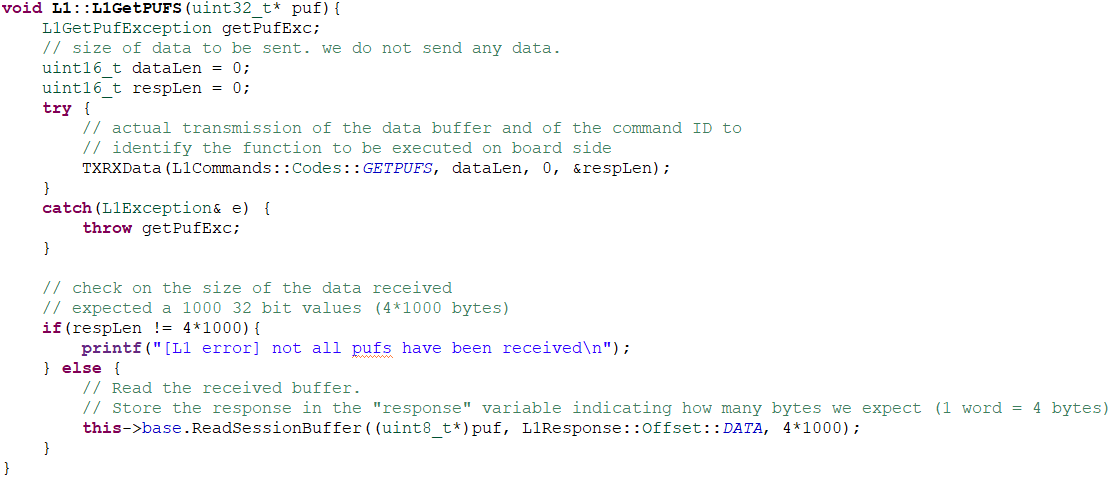
\includegraphics[width = 0.8\textwidth]{images/L1GetPUFS.png}
	\caption{Function responsible for communicating with the board and receiving the list of PUFs. }
	\label{fig:L1GetPUFS}
\end{figure}

In that piece of code we can see that we are expecting 1000 PUFs. The communication between host and board is done through the use of buffers that will then be transmitted using an appropriate transmit/receive function. In that buffer we must set the data to be sent and the size of the data we are transmitting/receiving. Then this buffer is sent with the command ID for the operation that must be performed on the board side. The response then will be given again through a buffer from which we can indicate where to store the result and the amount of bytes we expect. After that the host is responsible of managing that data, in our case to the write them in a DB.

\subsection{Board side}

In this stage the board is responsible of retrieving the initial data, PUFs, from the RAM and store them to the flash memory so that they can be accessed safely later.

Since the content of the RAM will be overwritten, the PUFs must be copied as soon as possible. For this reason this operation has to be done before any memory initialization. So this operation is done in the startup assembly file in which the reset handler can be found. This way we guarantee that we read the RAM before spoiling the RAM content which would mean compromising the PUFs.

Since the flash needs control registers to be set in order to be accessed in a safe way we relied on the HAL functions provided by STMicroelectronics. More precisely the functions to unlock and program/write in memory. The code written to perform this operation can be seen in figure \ref{fig:code_assembly}

\begin{figure}[h!]
	\centering
	\vspace{0.5cm}
	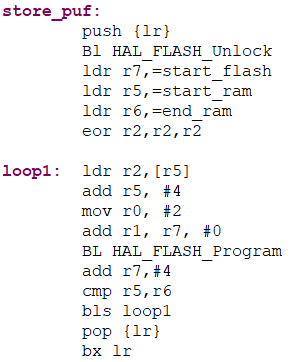
\includegraphics[width = 0.3\textwidth]{images/code_assembly.png}
	\caption{Assembly code to store PUFs into the flash memory. }
	\label{fig:code_assembly}
\end{figure}

Using the reference manual for the MCU STM32f429 we know the memory mapping of both the SRAM(0x020000000 -  0x02002FFFF) and flash memory(0x08000000 - 0x081FFFFF). Starting from that we scanned the SRAM and loaded the content to a part of the flash that will not overwrite sensible data.

At the end of the execution of the assembly code we expect 1000 PUFs to be stored in the flash memory which will be accessible once we enter the main.cpp and eventually the execution loop. At that point we can call the implemented functions and access the content of the flash.

Once we have the PUFs in memory we need access to them. This is done in the $puf\_retreive()$ function, found in the $se3\_dispatcher\_core.c$ file. This is the function associated to the command code transmitted from the Host side to the board.

To make the command call possible it is necessary to define these commands in the $se3\_dispatcher\_core.h$ which must reflect the ID associated to the same command found on the host side.

\begin{figure}[h!]
	\vspace{0.5cm}
	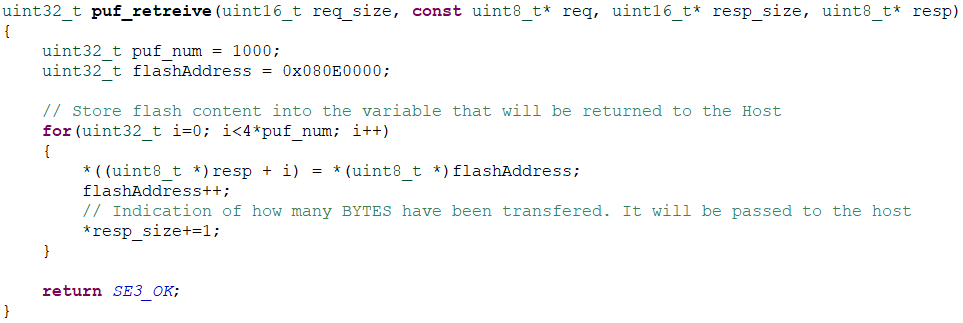
\includegraphics[width = 0.8\textwidth]{images/puf_retreive.png}
	\caption{puf\_retreive function. }
	\label{fig:puf_retreive}
\end{figure}

In the $puf\_retreive()$ function we simply read from the flash the PUFS that we stored at startup. This data is the data that will be sent to the host side.


\section {Application of a challenge and verification of the device} 
\label{section:impl_host}

Once we have the DB filled with the PUFs we can use it to check the authenticity of the board by comparing the PUFs in the DB to the ones provided by the board. Again to realize the functionality we will have to perform some tasks on the host and some on the board side.

\subsection{Host side}

The approach is similar to the one used for reading the PUFs but now we have different parameters to transmit. In fact we need to provide some data, the challenge, for the board to work on. So the Host is responsible of getting the challenge, use it to access the DB and retrieve the expected response. Then the challenge is sent to the board expecting in return the actual response to that challenge.

The next stage is to perform the actual transmit/receive which is done using the L1ChallengePUF function of the L1 API, see figure \ref{fig:L1ChallengePUF}.

\begin{figure}[h!]
	\vspace{0.5cm}
	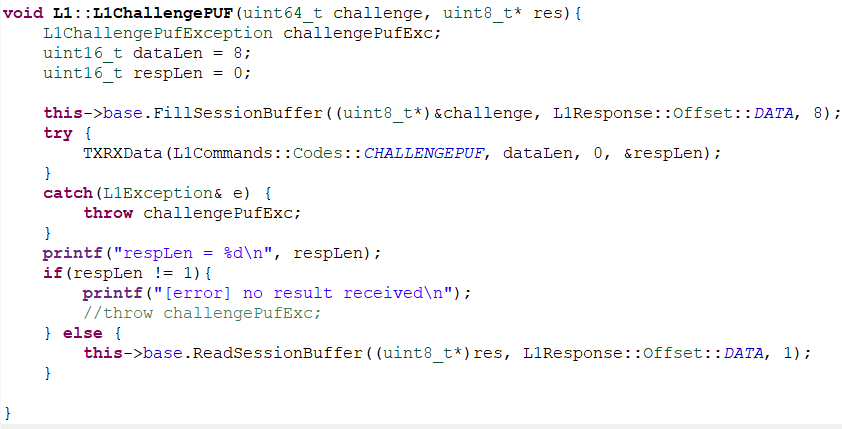
\includegraphics[width = 0.8\textwidth]{images/L1ChallengePUF.png}
	\caption{L1ChallengePUF function for transmitting challenge and response PUF}
	\label{fig:L1ChallengePUF}
\end{figure}


In this function we have some data to transmit and since the TXRX works on bytes, we have to provide the size of the data to be sent/received in bytes which is 4 since we transmit just 32bit of the challenge. Then as a response we expect just one 32bit value so another 4 bytes.

Once the Host has both expected and actual response it compares them using an acceptable Hamming distance. The one chosen is a distance of 4 bits. This choice is based on statistical results we obtained. These operations are done in the $examples > puf\_challenge.cpp$ file shown in figure \ref{fig:puf_challenge.cpp}

\begin{figure}[h!]
	\vspace{0.5cm}
	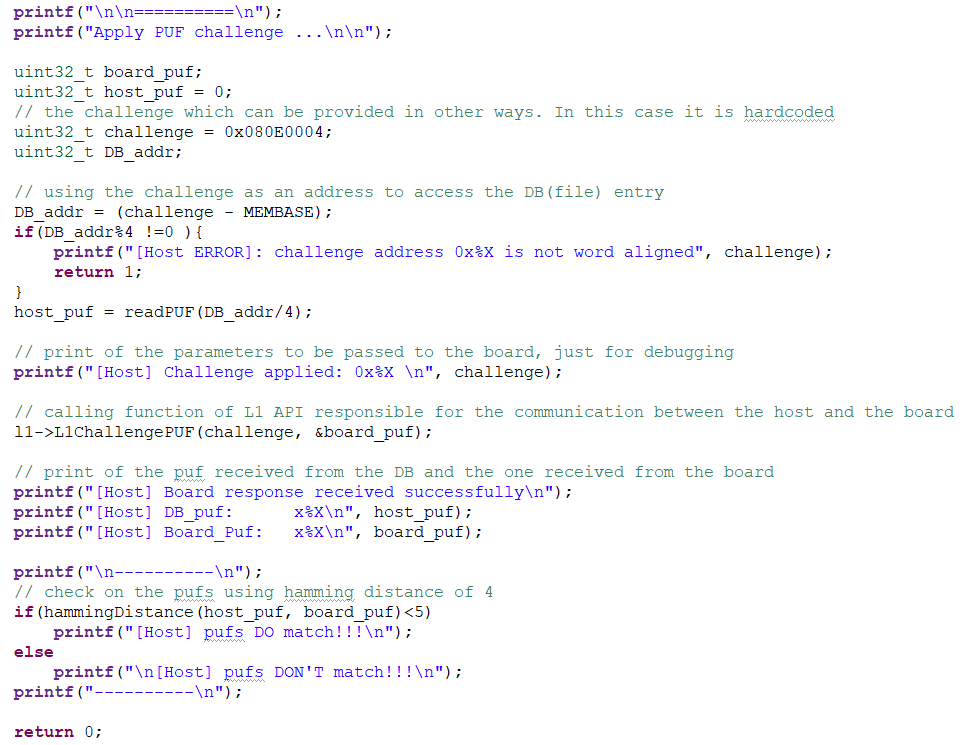
\includegraphics[width = 0.8\textwidth]{images/puf_challenge.png}
	\caption{puf\_challenge.cpp}
	\label{fig:puf_challenge.cpp}
\end{figure}

\subsection{Board side}

The Board at this point has been provided with the challenge. But the data has been sent using Little endian encoding so before being able to use the parameter passed a reconstruction is necessary.

So we reconstruct the data received to obtain the challenge. From there we can access the flash memory using the challenge as an address. This will be the actual PUF response returned to the Host.

\begin{figure}[h!]
	\vspace{0.5cm}
	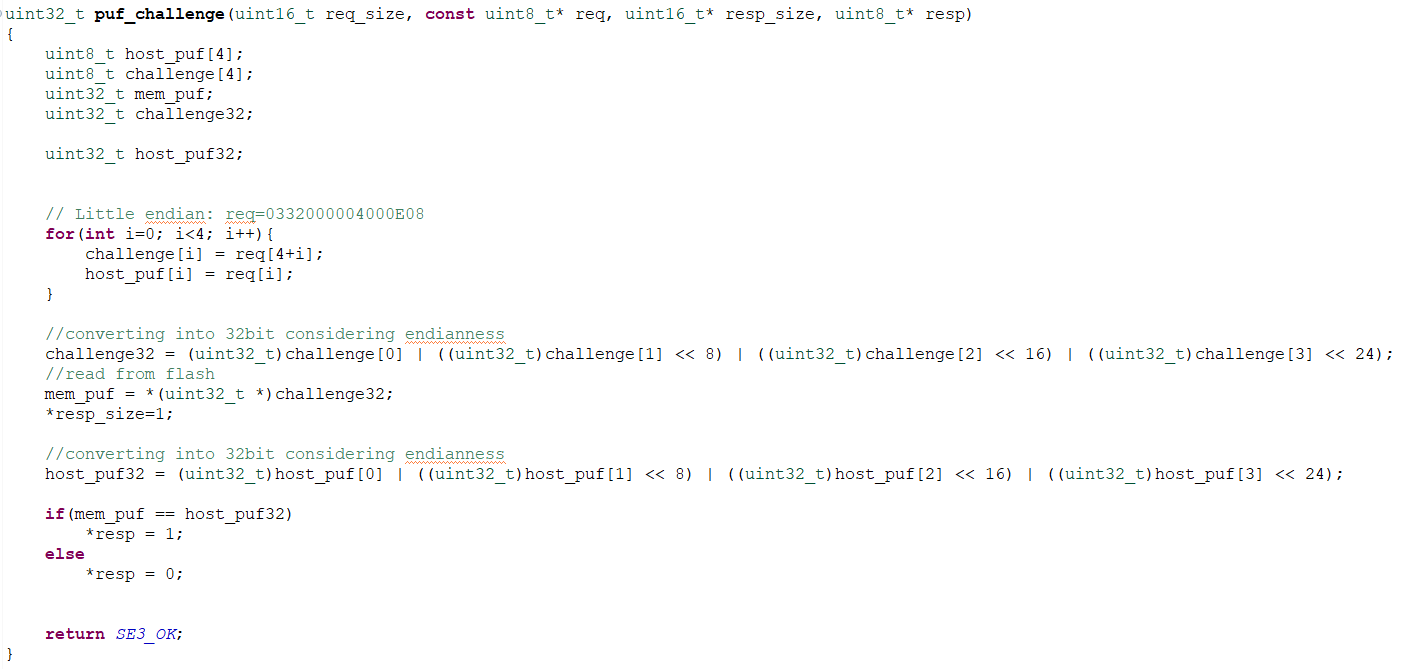
\includegraphics[width = 0.8\textwidth]{images/puf_challenge_board.png}
	\caption{puf\_challenge\_board function on the board side}
	\label{fig:puf_challenge_board}
\end{figure}

At this point the Board has completed its tasks and it is waiting for the next instruction. The Host on the other side will have to manage the response provided and complete the authentication process.